\documentclass[a4paper]{article}

%% Language and font encodings
\usepackage[english]{babel}
\usepackage[utf8x]{inputenc}
\usepackage[T1]{fontenc}

%% Sets page size and margins
\usepackage[a4paper,top=3cm,bottom=2cm,left=3cm,right=3cm,marginparwidth=1.75cm]{geometry}

%% Useful packages
\usepackage{amsmath}
\usepackage{graphicx}
\usepackage[colorinlistoftodos]{todonotes}
\usepackage[colorlinks=true, allcolors=blue]{hyperref}

\title{Using UPGMA on homonid mtDNA to test recent African origin hypothesis}
\author{William N. Bordowitz, Spencer Berg, Shaban Agayev, and Kai Ding}


\begin{document}
\maketitle
\nocite{globalalign}

\section{Introduction}

There is much debate over when in evolutionary time that humans (as they exist anatomically now) diverged from other primates. This requires us to take an ecological perspective of evolution, taking gene flow into consideration. In the recent African origin (RAO) hypothesis, modern humans arose roughly 100,000 years ago \cite{coolreview}
in Africa and migrated from there. Multiregionalism suggests that humans arose after multiple hominid populations migrated to multiple regions followed by substantial gene flow between the regions, creating a new species in the different regions semi-dependently. The multiregional hypothesis suggests that human evolution was the result of the rearranging of genes under strong selection and undergoing genetic drift, while the RAO hypothesis suggests a single speciation event that occurred.  \cite{fossils}

Phylogenetically, what this means is in the multiregional hypothesis, there is no single time that \textit{Homo sapiens} appeared, whereas the RAO hypothesis suggests the opposite. \cite{fossils} 

In any phylogenetic study of evolutionary distance a molecular clock is necessary. A commonly studied molecular clock in humans is in the mitochondrial genome. The mitochondrial genome provides genetic information that does not recombine, and as such is a better candidate for a molecular clock than autosomal sequences \cite{elsevierbs}.
This molecular clock has been known to provide accurate phylogenies when comparing human mtDNA sequences against other hominids. It is also important that a multiparameter distance metric be used in comparing the mtDNA sequences. 

According to a 2014 article by Rieux et al. the actual value of the entire human mitochondrial molecular clock is around $2.143 * 10^{-8} \frac{\frac{\mu}{site}}{year}$ with the highest variability at a region known as HVS1, with a value of $31.434 * 10^{-8} \frac{\frac{\mu}{site}}{year}$ \cite{mtdnastuff}.   
The mtDNA based human molecular clock was an improvement over the former methods that approximated distance by rough measures such as immunological distances. 
The distances found through the mitochondrial clock is more consistent with the fossil record, partially because they accounted for synonymous mutations, which are much more frequent then non-synonymous, and as such provided more recent dates for the human-ape split. There are several sites in the mitochondrial genome that have variable substitution rates, but those variances are typically mitigated when creating larger trees \cite{mtdnastuff}.

The sequencing of ancient genomes that have interbred or otherwise participated some sort of major gene-flow with the human genome the human genome (i.e Neanderthals, Denisovians, etc.) \cite{neanderthal} have provided insight into the timescale of early modern humans.The neanderthal genome, while there is a non-negligible amount of neanderthal genes in the human genome, diverged from the human mtDNA lineage around 300,000 years before the human ape split. The availability of completely sequenced ancient modern human mtDNA genomes provides a means of calculating more precise timescale of human evolution for researchers \cite{ancient}. These analyses have all pointed to a recent african origin. Additionally, the improvement of methods using larger data sets have for the most part been shown to suggest the validity of the RAO hypothesis \cite{penny}, and implies that the human-ape speciation event was the result of the fixation of various advantageous mutation in a predominant founding population \cite{multiregionalis}.
\section{Methods and results}

\subsection{Building the phylogeny}
The phylogenetic tree build from our program was constructed using UPGMA (discussed in the next section). This creates a bifurcating tree with a root that is rooted. We did this with bootstrapping to get a confidence interval for each of our clades. The downside of using UPGMA is that it creates an ultrametric tree, which assumes that the evolutionary distance from each branch to the root is the same, whereas in reality- despite these being mostly extant populations(neanderthals being the exception, of course)- they are likely not.
\subsection{Implementation}
Due to runtime concerns as well as memory concerns, an abridged version of the Mitochondrial genome was used. This likely affected the accuracy of our tree.

\subsubsection{Overview}
We used four steps during the implementation. The first step was global sequence alignment, which finds the best alignment of every two DNA pairs. Then we calculated the K2P distance among those DNA pairs and generated a distance matrix as the input of UPGMA. The third step was the UPGMA process, which found the minimum distance in the matrix and combined them together to get the new matrix until we got the final result. The output was a Newick tree format among those sequences. The final step was bootstrapping, which we randomly chose the bases from original DNA sequences and generate new input and go through all the steps again.

\subsubsection{global alignment}



\subsubsection{calculating K2P distance}
Our program calculates the K2P distances between each sequence in parallel. For each pair of sequences, global alignment was applied before counting the transitions and transversions in the aligned sequences. The final distance was calculated by $D_{K2P}=\frac{-1}{2} \ln(1 - 2 * S - V) - \frac{1}{4} \ln(1 - 2 * V)$, where $S$ is the ratio between the numbers of transitions and the length of the aligned sequence, and $V$ is the ratio between the numbers of transversions and the length of the aligned sequence.
\subsubsection{UPGMA}




\subsection{Results}
\begin{figure}
    \centering
    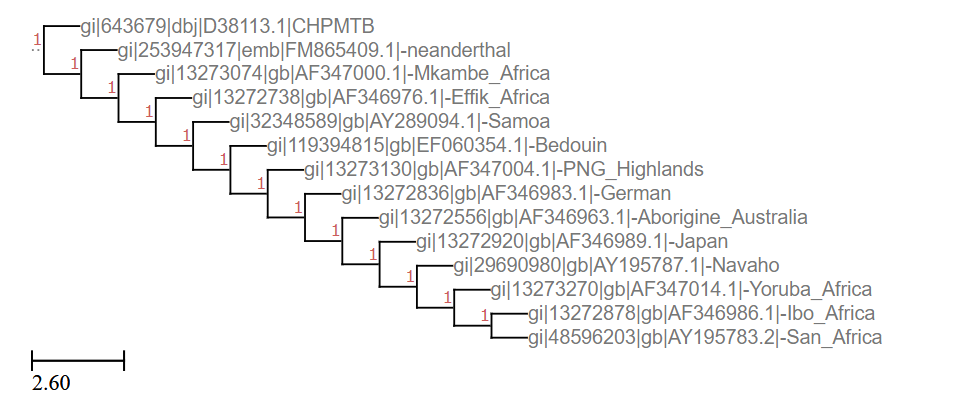
\includegraphics[scale=0.8]{bioinformatics.PNG}
    \caption{Tree output (rendered using ETE toolkit's Newick viewer)}
    \label{fig:my_label}
\end{figure}
This tree (Figure 1) shows that the MRCA of humans are most closely related to 2 native african populations. It is also likely that there was a trifurcation that was not caught due to the limitations of UPGMA, which led to 3 other African populations that were placed at the end of the phylogeny. Either way, the African populations are all grouped together on the phylogenetic tree which implies the validity of the RAO hypothesis, since that implies a single African founding population.


\bibliographystyle{ieeetr}
\bibliography{stuff}

\end{document}